\documentclass[11pt,letterpaper]{article}
\usepackage[top=0.67in,bottom=0.65in,left=0.75in,right=0.75in]{geometry}
\usepackage[T1]{fontenc}
\usepackage{lmodern,microtype}
\usepackage{amsmath,booktabs,tabularx,array,enumitem,xcolor,tikz,fancyhdr,hyperref}
\usetikzlibrary{arrows.meta,positioning}
\definecolor{ink}{HTML}{202C35}
\definecolor{accent}{HTML}{245D70}
\definecolor{muted}{HTML}{58636C}
\definecolor{pale}{HTML}{EDF3F5}
\definecolor{line}{HTML}{CCD9DE}
\hypersetup{colorlinks=true,urlcolor=accent,linkcolor=accent,
 pdftitle={SONIC: Professor meeting review notes},
 pdfauthor={Prepared for Howard Wang},pdfsubject={Flight study guide to the saved SONIC bioRxiv v1 preprint}}
\setlength{\parindent}{0pt}
\setlength{\parskip}{4pt}
\setlength{\tabcolsep}{5pt}
\renewcommand{\arraystretch}{1.16}
\setlist[enumerate]{leftmargin=18pt,itemsep=4pt,topsep=3pt,parsep=0pt}
\setlist[itemize]{leftmargin=14pt,itemsep=3pt,topsep=3pt,parsep=0pt}
\newcolumntype{L}{>{\raggedright\arraybackslash}X}
\pagestyle{fancy}\fancyhf{}
\fancyfoot[L]{\footnotesize\color{muted}SONIC review notes\enspace /\enspace Howard Wang\enspace /\enspace 14 October 2026}
\fancyfoot[R]{\footnotesize\color{accent}\thepage\ / 5}
\renewcommand{\headrulewidth}{0pt}\renewcommand{\footrulewidth}{0.3pt}
\setlength{\footskip}{24pt}
\newcommand{\pagehead}[3]{
 {\small\bfseries\color{accent}#1}\par\vspace{2pt}
 {\fontsize{23}{26}\selectfont\bfseries\color{ink}#2}\par
 {\color{muted}#3}\par\vspace{4pt}}
\newcommand{\topic}[1]{\vspace{5pt}{\large\bfseries\color{ink}#1}\par\vspace{1pt}}
\newcommand{\src}[1]{\par{\fontsize{8.5}{10}\selectfont\color{muted}Paper: #1\par}}
\newcommand{\takeaway}[1]{\par\vspace{3pt}\begingroup\setlength{\fboxsep}{8pt}
 \colorbox{pale}{\parbox{\dimexpr\linewidth-16pt\relax}{#1}}\endgroup\par\vspace{3pt}}
\newcommand{\smallnote}[1]{{\small\color{muted}#1\par}}
\begin{document}\color{ink}

\pagehead{01 / THE EXPERIMENT}{What is SONIC measuring?}{A reading guide for the professor meeting on 15 October 2026}

SONIC asks: \textbf{how much information about a known sound sequence can we recover from brain recordings, and with what delay?} Its name means \textit{Standard for Optimizing Neural Interface Capacity}.

\begin{center}
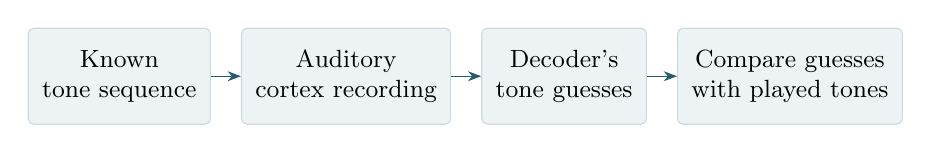
\begin{tikzpicture}[node distance=0.15in,box/.style={draw=line,fill=pale,rounded corners=2pt,align=center,font=\small,minimum height=0.48in,inner sep=5pt},>=Stealth]
\node[box] (a) {Known\\tone sequence};
\node[box,right=of a] (b) {Auditory\\cortex recording};
\node[box,right=of b] (c) {Decoder's\\tone guesses};
\node[box,right=of c] (d) {Compare guesses\\with played tones};
\draw[->,accent] (a)--(b);\draw[->,accent] (b)--(c);\draw[->,accent] (c)--(d);
\end{tikzpicture}
\end{center}
\src{\S2, Fig.\,1, pp.\,4--5}

\topic{The paper's animals and sessions}
Two \textbf{awake, alert sheep}, C and E, each had a 421-channel Connexus system in left primary auditory cortex (A1). Each animal had one exploratory session, then four benchmark sessions. They were selected from a larger cohort for the greatest estimated A1 coverage. This is a small, selected sample.
\src{\S3, p.\,5; \S6.6--6.7, p.\,13}

\topic{A tone is a short pip; frequency is its pitch}
A pip is a pure sine-wave sound. In the main benchmark, every pip lasts \textbf{10 ms}. The next pip starts immediately. The computer chooses a frequency from a fixed list; neighboring choices can repeat. There is no fixed repeating melody.

\begin{center}
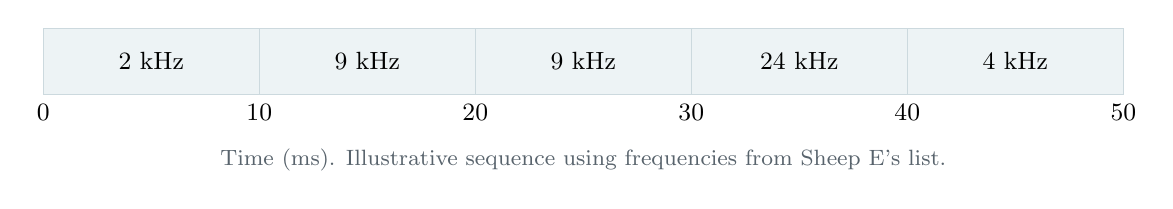
\begin{tikzpicture}[x=1.08in,y=0.3in,font=\small]
\foreach \x/\t in {0/2 kHz,1/9 kHz,2/9 kHz,3/24 kHz,4/4 kHz}{
 \draw[fill=pale,draw=line] (\x,0) rectangle (\x+1,1.1);
 \node at (\x+0.5,0.55) {\t};}
\foreach \x/\t in {0/0,1/10,2/20,3/30,4/40,5/50}{\node[below] at (\x,0) {\t};}
\node[below,font=\footnotesize\color{muted}] at (2.5,-0.75) {Time (ms). Illustrative sequence using frequencies from Sheep E's list.};
\end{tikzpicture}
\end{center}

\textbf{100 slots per second} comes from $1/0.010$. It does not mean 100 different pitches per second. A 2 kHz pip oscillates 2,000 times per second while it lasts: about 20 cycles in 10 ms.

{\small\begin{tabularx}{\linewidth}{@{}p{1.42in}p{1.21in}L@{}}
\toprule
\textbf{Quantity} & \textbf{Paper value} & \textbf{What it counts}\\\midrule
Sound frequency & kHz & Wave cycles per second: pitch\\
Tone presentation & 100/s & 10 ms slots: stimulus choices\\
Audio DAC rate & 192,000 samples/s & Electrical waveform samples\\
Neural sample rate & 5,200/s/channel & Voltage measurements on each channel\\
Feature bin & 5 ms & Time grouped into one neural summary\\
Recovered ITR & bits/s & Information retained in the predictions\\\bottomrule
\end{tabularx}}
\src{\S6.1--6.3, p.\,11; \S6.5, p.\,12. Slot rate and cycle count are derived.}

\smallnote{\textbf{Optional detail: neural recording settings.} Analog band $\sim$10 Hz--2.2 kHz; digital high-pass $\sim$300 Hz, rolling 5 ms zero-phase filter, then common-average reference (subtract the shared channel average). Events cross $-3\times$ RMS (a measure of voltage size), estimated from the first 2 s, with a minimum 1 ms interval. These are paper settings, not universal requirements. Features are explained on page 2. (\S6.3, p.\,11.)}

\smallnote{Source throughout: Perkins et al., \textit{SONIC: A Benchmarking Paradigm for Brain-Computer Interfaces}, saved bioRxiv v1, posted 2 October 2025. \href{https://doi.org/10.1101/2025.09.30.679683}{DOI: 10.1101/2025.09.30.679683}. References use the saved PDF's page numbers. This guide does not establish current publication status.}

\newpage
\pagehead{02 / SOUND TO PREDICTION}{How does the test work?}{The sound is prepared first; the decoder learns from labeled recordings.}

\begin{center}
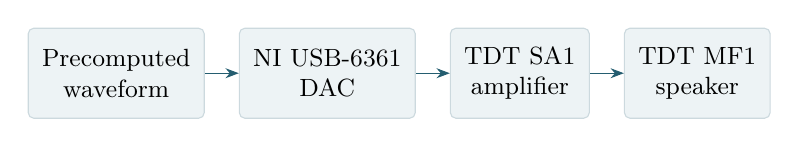
\begin{tikzpicture}[node distance=0.17in,box/.style={draw=line,fill=pale,rounded corners=2pt,align=center,font=\small,minimum height=0.45in,inner sep=5pt},>=Stealth]
\node[box] (a) {Precomputed\\waveform};
\node[box,right=of a] (b) {NI USB-6361\\DAC};
\node[box,right=of b] (c) {TDT SA1\\amplifier};
\node[box,right=of c] (d) {TDT MF1\\speaker};
\draw[->,accent] (a)--(b);\draw[->,accent] (b)--(c);\draw[->,accent] (c)--(d);
\end{tikzpicture}
\end{center}

The \textbf{DAC} turns stored numbers into an electrical waveform. The \textbf{amplifier} supplies the drive for the \textbf{speaker}, which turns it into sound. The same speaker changes pitch when the waveform changes; nobody switches it manually. Each pip starts at zero phase and has 2 ms amplitude ramps at both ends, included in its duration, to reduce clicks. The ramp shape is unspecified.

The paper reports approximately \textbf{80 dB SPL at sheep-ear distance}. This is a reported condition, not a Rice exposure prescription. Exact geometry and frequency-by-frequency calibration details are absent. A measurement microphone checks what arrives at the ear position; the neural recorder measures brain voltages. A high DAC rate alone does not establish the speaker's or microphone's usable acoustic band.
\src{\S6.2--6.3, p.\,11. Microphone role is an engineering explanation.}

\topic{What sounds did they choose?}
Sheep C kept 37 frequencies, described as 1/8-octave steps over about 1.4--32 kHz. The exact 37-value array is absent. Sheep E used 14 refined choices after exploration showed which pitches its implant distinguished well: 2, 4, 6, 8, 9, 10.5, 17, 18.2, 19.5, 20.9, 22.4, 24, 25.8 and 27 kHz.

Frequencies were random, uniform and balanced at the block level. The seed and exact balancing algorithm are unspecified. A block held 8,000--15,000 tones: \textbf{80--150 s of sound} at 10 ms, then 1 s silence between blocks. At least 12 blocks were collected per session; this is not an exact full-session duration. Exploration tested 4--24 ms in 2 ms steps; Fig.\,2 and Methods disagree about duration grouping.
\src{Figs.\,2--3, p.\,6; \S6.1, p.\,11. Block seconds are derived.}

\topic{What enters the decoder?}
For every channel, the paper made two summaries in each 5 ms bin:
\begin{itemize}
\item \textbf{Spike count:} the number of sufficiently negative threshold crossings. These are detected events, not proof of separately identified single neurons.
\item \textbf{Spike-band power:} average squared filtered voltage, measuring the strength of that fast electrical activity.
\end{itemize}
The main model uses ten bins spanning \textbf{10--60 ms after each tone onset}. Because tones start every 10 ms, adjacent tones' 50 ms windows overlap.
\src{\S6.3, p.\,11}

\topic{How is a guess judged fairly?}
Training pairs a known tone label with its neural pattern. Validation helps choose the model; a separate test set judges it. The main two-layer 1D convolutional network used 400 units per layer, kernel 5 and stride 1.

The paper used 8--16 folds and kept whole contiguous blocks together, avoiding shared windows across train/test boundaries. Test predictions were pooled across folds. Preprocessing must keep test data out of fitting; the paper's normalization used a subset of training plus validation data. \textbf{Exact correct} means the guessed frequency equals the played frequency. There is no universal pass/fail accuracy.
\src{\S6.4, p.\,12. Pass/fail statement is interpretation.}

\newpage
\pagehead{03 / BITS AND RESULTS}{What does ITR mean?}{A bit measures uncertainty removed, not a spike or a sample.}

Perfectly identifying two equally likely choices conveys \textbf{1 bit}; four conveys \textbf{2 bits}: two yes/no answers identify one of four. Independent guesses convey zero information about the played tone.

\topic{Worked example: wrong guesses can still help}
\smallnote{Illustrative population example, not paper or Rice data. Four equally likely tones.}
{\small\begin{tabularx}{\linewidth}{@{}p{1.43in}*{4}{>{\centering\arraybackslash}X}@{}}
\toprule
Tone played & A & B & C & D\\
Decoder predicts & A & A & C & C\\
Exactly correct? & Yes & No & Yes & No\\\bottomrule
\end{tabularx}}

The decoder is exactly right only \textbf{50\%} of the time. Yet every prediction tells us the correct pair: A/B or C/D. Four possibilities shrink to two. That preserves \textbf{1 bit per tone}. At a hypothetical 100 independent tones/s, that is \textbf{100 bits/s}. This uses exact population probabilities; no finite-sample correction is applied.

\takeaway{\textbf{Accuracy asks whether the exact label was right.} Information asks how much the guess tells us. Different error patterns can preserve different information, even with the same accuracy and number of choices.}

\topic{The paper's calculation, in three steps}
\begin{enumerate}
\item Count presented versus predicted tones in a \textbf{confusion matrix}. Rows are played tones; columns are predictions. Its diagonal counts exact matches.
\item Compute \textbf{mutual information}: how much knowing the prediction reduces uncertainty about the played tone. Subtract the paper's finite-sample bias correction.
\item Divide corrected bits per tone by tone duration in seconds. At 10 ms, multiply by 100.
\end{enumerate}
\vspace{-3pt}
\[
 \mathrm{ITR}=\frac{I_{\mathrm{corrected}}}{\tau},\qquad
 I_{\mathrm{corrected}}=I-\frac{(K-1)^2}{2N\ln 2}.
\]
\smallnote{$K$ = number of tone classes; $N$ = pooled held-out predictions; $\tau$ = tone duration in seconds. Accuracy alone cannot calculate $I$; accuracy $\times\log_2 K$ is not this method.}
\src{\S6.5, p.\,12}

\topic{What the main benchmark achieved}
{\small\begin{tabularx}{\linewidth}{@{}p{0.48in}p{0.58in}p{1.32in}L L@{}}
\toprule
\textbf{Sheep} & \textbf{Choices} & \textbf{Exact accuracy} & \textbf{Mean achieved ITR} & \textbf{Perfect input ceiling}\\\midrule
C & 37 & $45.4\%\pm3.1\%$ & 201.9 bits/s & $\sim$521 bits/s\\
E & 14 & $75.9\%\pm0.7\%$ & 230.1 bits/s & $\sim$381 bits/s\\\bottomrule
\end{tabularx}}
\smallnote{Four benchmark sessions per sheep; accuracy is mean $\pm$ session SD. Ceilings assume uniform tones and perfect recovery: $\log_2(K)/0.010$. They are theoretical, not achieved rates.}
\src{\S3, Table\,1 and text, p.\,7}

The reported means imply \textbf{2.019 and 2.301 corrected bits/tone} (divide by 100), not newly reproduced raw-data results. Each mean exceeded 200 bits/s; not every session did. This rate omits silence, calibration and training; whole-session throughput differs.

Achieved ITR depends on stimuli, site, processing and decoder. Sensory decoding does not establish voluntary communication, speech decoding, intelligence or full brain/device capacity. Two selected animals and no matched-device comparison limit generality.
\src{\S3, p.\,7; \S4.1--4.3, pp.\,9--10; \S6.5, p.\,12. Bits/tone and wall-clock notes are derived.}

\newpage
\pagehead{04 / TIMING}{How fast is the answer?}{Throughput, waiting time and timestamp uncertainty are different.}

\topic{The observation window overlaps later tones}
\begin{center}
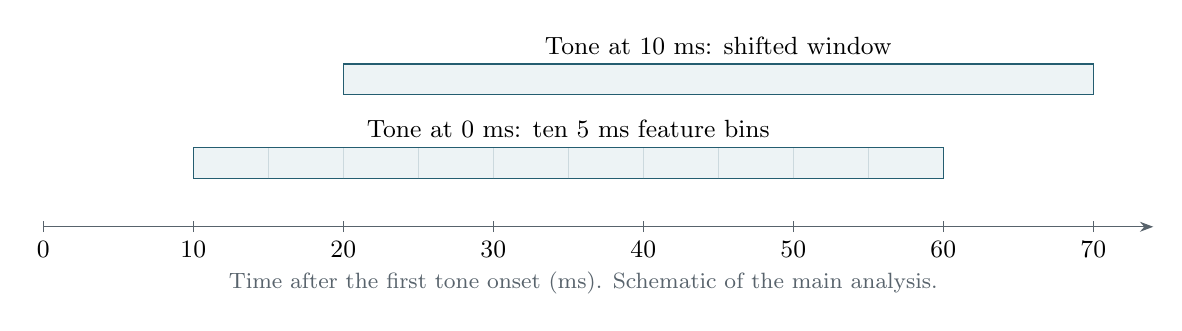
\begin{tikzpicture}[x=0.075in,y=0.22in,font=\small,>=Stealth]
\draw[->,muted] (0,0)--(74,0);
\foreach \x in {0,10,20,30,40,50,60,70}{\draw[muted] (\x,-0.12)--(\x,0.12);\node[below] at (\x,-0.12) {\x};}
\draw[fill=pale,draw=accent] (10,1.1) rectangle (60,1.8);
\foreach \x in {15,20,25,30,35,40,45,50,55}{\draw[line] (\x,1.1)--(\x,1.8);}
\node[above] at (35,1.8) {Tone at 0 ms: ten 5 ms feature bins};
\draw[fill=pale,draw=accent] (20,3) rectangle (70,3.7);
\node[above] at (45,3.7) {Tone at 10 ms: shifted window};
\node[below,font=\footnotesize\color{muted}] at (36,-0.8) {Time after the first tone onset (ms). Schematic of the main analysis.};
\end{tikzpicture}
\end{center}
The 10--60 ms window is 50 ms long. Later tones play during it. This observation span is not a 60 ms intrinsic-delay term to add to 56 ms.
\src{\S3, p.\,7; \S6.3, p.\,11}

\topic{What the reported 56 ms includes}
{\small\begin{tabularx}{\linewidth}{@{}p{1.55in}p{0.65in}L@{}}
\toprule
\textbf{Component} & \textbf{Delay} & \textbf{Plain meaning}\\\midrule
Neural measurement & $<1$ ms & Recording hardware makes activity available\\
Filtering & 5 ms & Buffered signal processing\\
Latest feature bin & 5 ms & Collect one bin's worth of data\\
Earlier context & 45 ms & Collect the other nine bins\\\bottomrule
\end{tabularx}}

The reported \textbf{56 ms intrinsic delay} excludes sound-to-response physiology and computer runtime. Its listed components sum to less than 56 ms (reporting/rounding convention). The displayed analyses were offline; a separate online neural-interface-plus-compute evaluation reports less than 100 ms, also excluding physiology.
\src{\S2, pp.\,4--5; \S3, p.\,7; \S4.1, p.\,9}

\topic{What the 11 ms result means}
Figure 5's more than 100 bits/s at 11 ms intrinsic delay uses one 5 ms bin. It covers \textbf{only the first 40\% of Sheep E, Session 2}, one 75/12.5/12.5\% train/validation/test split, and a one-layer, kernel-1 model. The curve maximizes over window alignments. This is a narrower sweep, not the main eight-session result or sound-onset-to-answer latency.
\src{Fig.\,5, p.\,8; \S6.4, p.\,12}

\topic{Three timing questions for our setup}
\textbf{Latency:} waiting time for output. \textbf{Alignment error:} uncertainty placing sound on the neural timeline. \textbf{Drift:} mismatch growing over time. A known delay can be corrected while leaving small uncertainty. One shared start trigger does not establish equal clock speeds.

The paper synchronized audio and Connexus using PTP (network time) and 10 MHz, recording electrical output and trial-start edges. Residual acoustic alignment error and drift are unquantified. Rice needs compatible recorder inputs plus electrical and acoustic onset measurements.
\src{\S6.2, p.\,11. Timing distinctions and Rice checks are engineering interpretation.}

\newpage
\pagehead{05 / THE MEETING}{What should we decide first?}{Use the existing equipment list to discuss functions and missing evidence.}

\topic{Seven questions, in priority order}
\begin{enumerate}
\item \textbf{First success criterion.} Start with a reliable sound-evoked response, or tone classification and ITR? What result would count as success?
\item \textbf{Preparation.} Which species and preparation come first? Reconfirm awake/sedated state and recording site. The paper used awake, alert sheep; reconfirm Rice's state.
\item \textbf{Frequency set.} Start with a selected audible subset or the full paper band? Which tones matter for our preparation and recording site?
\item \textbf{Sound at the ear.} Agree on target SPL, equal measured level across frequencies versus deliberate level variation, calibration method/tolerance, speaker geometry, background sound, and session/exposure settings with the lab.
\item \textbf{Recording and alignment.} Which recorder/software and auxiliary analog, digital and clock inputs exist? How will we measure sound-to-neural alignment, acceptable uncertainty and drift?
\item \textbf{Available equipment.} What do we own or can we borrow? Which items are only BCM suggestions? Confirm the budget against the existing options.
\item \textbf{Next milestone.} Agree on one animal-free bench deliverable, its owner, date and required evidence.
\end{enumerate}

\takeaway{\textbf{Proposed bench milestone:} save a tone sequence; measure each frequency at the planned ear position; capture playback markers and microphone sound on an aligned timeline; report level variation, onset uncertainty and drift over a representative run. Agree on tolerances first. This bench work remains to be done.}

\smallnote{Recorded project direction does not require a soundproof box or behavioral rig. Background sound, repeatable geometry and calibration still matter. Rice hardware availability, calibrated playback, bench results and neural results remain unverified. This guide is study material, not an animal-ready protocol.}

\topic{Quick glossary}
{\small\begin{tabularx}{\linewidth}{@{}p{1.0in}L p{0.65in}L@{}}
\toprule
\textbf{A1} & Primary auditory cortex & \textbf{DAC} & Digital-to-analog converter\\
\textbf{SPL} & Sound pressure level & \textbf{Bin} & Short time interval summarized\\
\textbf{Label} & Known tone identity & \textbf{Fold} & One data partition\\
\textbf{Bit} & Unit of information & \textbf{ITR} & Recovered information per second\\\bottomrule
\end{tabularx}}

\topic{Cover the answers and check recall}
{\small
\textbf{1.} A 10 ms pip is 9 kHz. Is the tone rate 9,000/s?\quad
\textbf{2.} Does 50\% exact accuracy always mean zero information?\quad
\textbf{3.} Why keep whole blocks together when testing?\quad
\textbf{4.} Is 56 ms the paper's acoustic synchronization error?\quad
\textbf{5.} What does 230.1 bits/s mean at 100 tone slots/s?

\textbf{Answers.} \textbf{1.} No: 9 kHz is pitch; 10 ms slots give 100 tones/s. \textbf{2.} No: the pair example retains 1 bit/tone. \textbf{3.} Adjacent windows overlap; splitting them can leak data. \textbf{4.} No: it is intrinsic processing/aggregation delay, excluding physiology and compute. \textbf{5.} An average of 2.301 corrected bits/tone, not 230.1 exact tone identifications per second.
}

\vfill
{\fontsize{8.5}{10}\selectfont\color{muted}
\textbf{Source and scope.} Perkins et al., saved \href{https://doi.org/10.1101/2025.09.30.679683}{SONIC bioRxiv v1} (2 October 2025). Original PDF unchanged, CC BY-NC-ND 4.0. This guide contains independent notes and original schematic diagrams. Project context: \href{https://github.com/HowardWHSrun/audiotory_benchmark/blob/main/sources/Team_Clarifications_2026-10-07.md}{recorded team direction} and \href{https://github.com/HowardWHSrun/audiotory_benchmark/blob/main/output/pdf/Auditory_Hardware_Options_2026-10-09.pdf}{existing equipment/options list}; confirm local availability and preparation.}

\end{document}
